\section{Introduction}
Approximate Nearest Neighbor Search (ANNS) is a core primitive in modern data systems, including Retrieval-Augmented Generation (RAG), 
recommendation, and anomaly detection~\cite{Zhong20255017}. Among existing ANNS index families, graph-based indices such as HNSW~\cite{Jayaram2019, Malkov2020824} are 
widely adopted because they offer strong recall-latency trade-offs at scale. Their search process relies on iterative graph traversal from 
vertices to their neighbors, where random memory access and cache misses often dominate query latency in practice. To mitigate these challenges, prior work has explored a broad range of optimizations: some efforts make distance computation and traversal faster through optimized storage layout, quantization techniques, etc~\cite{Gou2025, Wang2025, Zhong20255017}, while others reduce the amount of computation through pruning and distance estimation~\cite{Chen20233225, Gao202327, Song2025}.

Despite substantial progress, most existing optimizations are developed for static snapshots. In reality, vector data are continuously inserted and deleted \cite{Gong20251593,Wang202627}, causing the index topology and data distribution to evolve over time.
This leads to a temporal mismatch: \textbf{\textit{pre-computed search hints}}, i.e., auxiliary information or structures used to accelerate queries, may be 
effective at time $t$ but become stale at time $t+\Delta$, reducing alignment with the current index and degrading query efficiency.
The effect is especially severe in high-rate ingestion workloads, where updates arrive continuously and drift accumulates quickly. A representative case is real-time payment fraud detection~\cite{microsoft2025fraud, aws2024memorydbvector}, where incoming transactions are embedded and matched against a continuously updated behavioral database via ANNS under millisecond-level decision SLAs.
In such systems, the index must absorb new transactions while serving latency-critical queries. 
Significant performance degradation across updates is unacceptable because delayed retrieval directly increases fraud leakage risk and financial loss.

\begin{figure}
	\centering
	\subfloat[One-shot optimization]{
		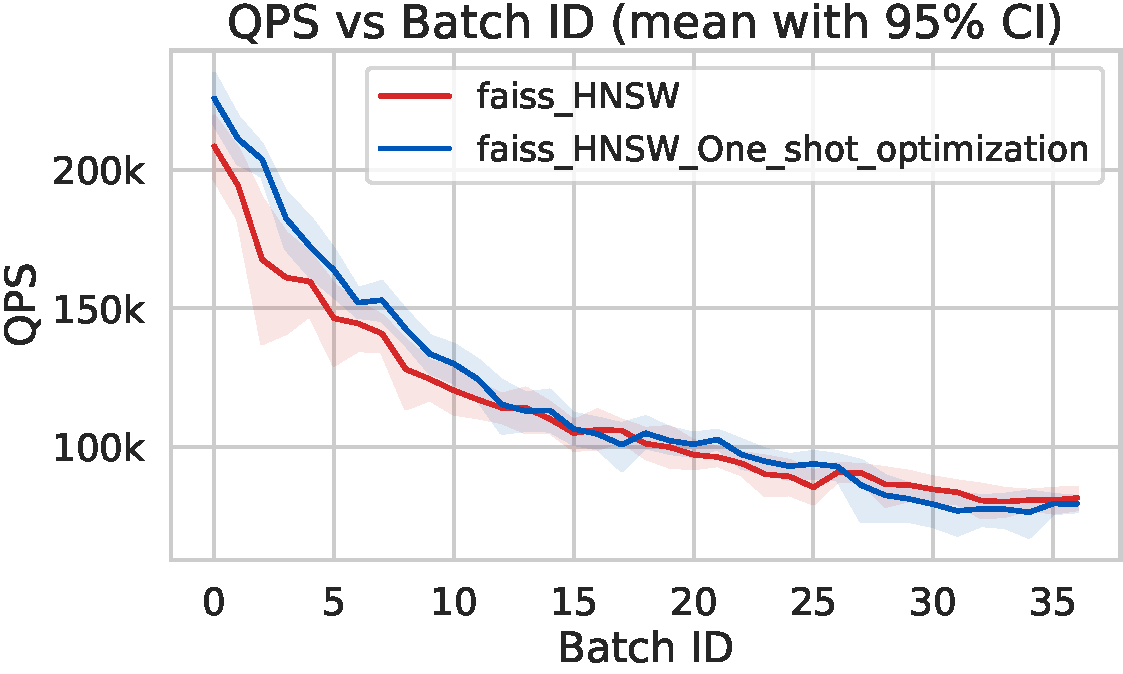
\includegraphics[width=0.48\columnwidth]{figures/figure1a.pdf}
		\label{fig:stale-hint}
	}
    \subfloat[Frequent re-optimization]{
		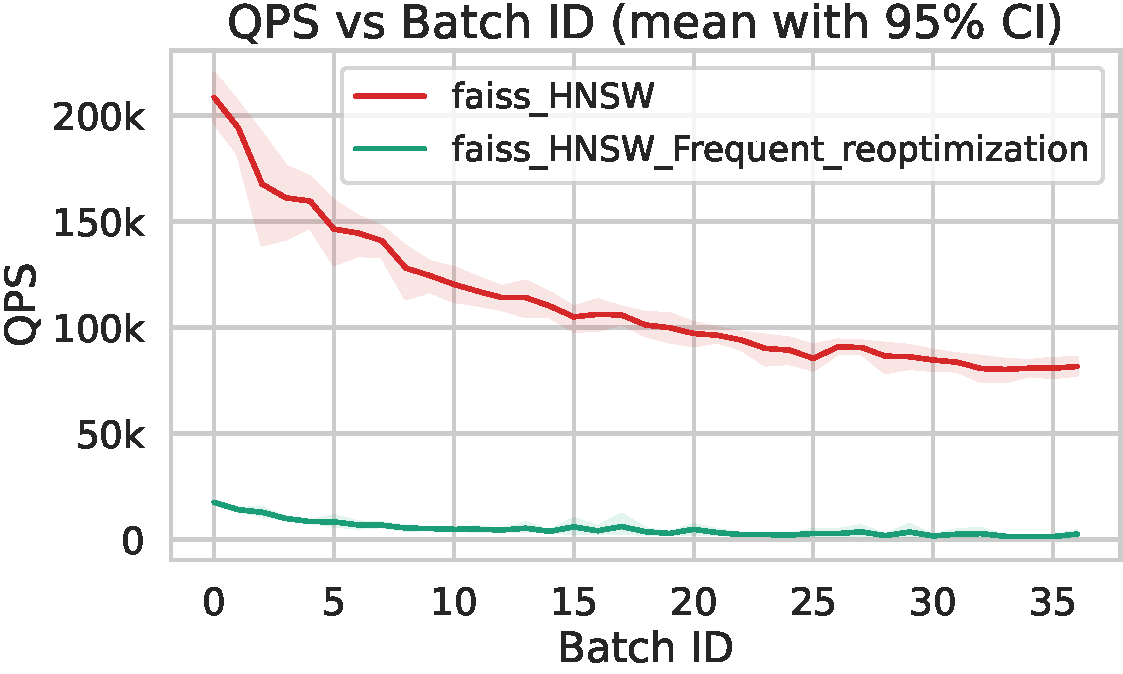
\includegraphics[width=0.48\columnwidth]{figures/figure1b.pdf}
		\label{fig:reopt-cost}
	}
    \caption{Trade-offs in dynamic ANNS: one-shot optimization provides only short-term gains, while aggressive frequent re-optimization hurts overall query throughput, tested on \cite{Coleman202238488}.}
	\label{fig:motivation}
\end{figure}

To alleviate update-induced performance decay, dynamic ANNS faces a fundamental efficiency-maintenance dilemma, as illustrated in Figure~\ref{fig:motivation}. If search hints are computed once and left 
unmaintained during updates, they may provide short-term gains in early rounds, but their benefit decays over time, causing query throughput to progressively fall back toward baseline performance (Figure~\ref{fig:stale-hint}). In contrast, if the system frequently 
rebuilds or globally re-optimizes them, the maintenance overhead is prohibitive and can dominate end-to-end runtime, limiting overall throughput gains (Figure~\ref{fig:reopt-cost}). Consequently, the key challenge is not merely how 
to accelerate search, but how to keep acceleration \emph{continuously valid} under ongoing updates without incurring prohibitive maintenance cost. To our knowledge, no existing work has designed search hints or query acceleration mechanisms that remain effective in such dynamic settings.


In this paper, we present \system, an index-agnostic plugin for continuously accelerating ANNS query performance under dynamic updates. The key observation behind \system is that historical search outcomes do not lose their utility uniformly after updates. In many dynamic workloads, batch queries still exhibit substantial top-$k$ overlap across update rounds, query accesses are often highly skewed, and different queries may have different degrees of result stability. Based on these observations, \system selectively reuses past successful search outcomes as lightweight search states, called \textit{seeds}, to avoid repeatedly executing queries from scratch. Unlike existing search hints, seeds are designed to be maintained online to trace index changes over time. As a result, seeds provide update-aware guidance for candidate generation across update rounds without resorting to one-shot offline optimization or frequent global re-optimization.
This approach reduces redundant graph traversal and distance computation, yielding higher end-to-end query efficiency under dynamic updates.

A key design in \system is to organize seed reuse as an online store--retrieve--validate workflow.
First, \system maintains a compact two-tier seed storage, where each \textit{seed} records historical results together with lightweight freshness and utility signals.
The high-utility layer keeps a small set of valuable seeds for fast access, while the semantic-shared layer provides bounded coverage for long-tail historical results.
Second, at query time, \system retrieves seeds through exact-key lookup and signature-based scan over high-utility seeds or signature-based probing over semantic-based seeds, and uses the retrieved seeds to guide bounded neighbor expansion and candidate generation. Third, before returning the seed-guided top-$k$ results, \system applies a lightweight validation gate; if reuse is unreliable, the query falls back to the original backend search procedure.
After each processing round, effective seeds are selectively written back, and low-value seeds are evicted, allowing the seed storage to track workload skew and index drift with bounded maintenance overhead.

Different from existing static ANNS optimizations, \system focuses on sustaining query-throughput gains as the index continuously evolves under updates. \system is also complementary to existing dynamic ANNS works \cite{Singh2021,Liu20252268,Voruganti2025} that primarily optimize update throughput or graph maintenance. \system operates as a pluggable post-update query acceleration layer, decoupled from backend-specific graph internals. We evaluate \system on CANDOR-Bench~\cite{Wang202627}, a streaming ANNS benchmark, across three state-of-the-art ANNS backends, where it improves query throughput by 1.47x--3.34x. Our code is available at https://github.com/intellistream/CANDOR-Bench/tree/BriskSeed.

%{\color{blue}To address this challenge, we propose \system, an ANNS plugin for continuously accelerating query throughput under dynamic updates.}Our design is motivated by two observations. First, for batch queries, top-$k$ result sets often remain substantially overlapped under moderate updates, indicating that historical search states may still retain reuse value. Second, query access frequencies are highly skewed, and a small fraction of vectors account for a large fraction of accesses, making it possible to maintain reusable search states in a compact and selective manner.
%{\color{blue} Instead of xxx, \system designs a seed healing. First seed storage   Second seed reuse  Third seed  validation}
%Based on these observations, \system converts one-shot offline optimization into an online reuse--validate--refresh loop over historical search states. The main design challenge is to maintain reusable search states compactly as the index evolves, determine when a historical state can still be reused safely, and refresh or reject it with sufficiently low overhead so that maintenance cost does not offset the acceleration benefit. To this end, \system maintains a two-tier seed storage, where each \textit{seed} records historical results together with lightweight freshness and utility signals. At query time, \system first attempts reuse from a hot-exact tier and otherwise falls back to a semantic-shared tier. The retrieved seed is then used for bounded neighbor expansion to recover candidate results, which are accepted as the new top-$k$ only if they pass a validation gate; otherwise, the query falls back to the baseline search. After each round, effective seeds are selectively written back, and low-value ones are evicted, allowing the seed storage to track workload and index drift without global rebuilding. As a result, \system improves end-to-end query efficiency while preserving recall under dynamic updates. To keep deployment practical, \system decouples its control logic from backend-specific index internals, enabling low-effort integration with existing dynamic ANN backends.



This paper makes the following contributions:
\begin{itemize}
\item We identify stale auxiliary guidance as a major cause of search-efficiency decay in dynamic ANNS, and formulate the problem as an amortized trade-off between search acceleration and guidance maintenance.
\item We present \system, an ANNS plugin to improve query performance under dynamic updates by using seeds, while remaining decoupled from 
backend-specific index internals.
\item We evaluate \system on CANDOR-Bench through extensive experiments. The results show that \system enhances end-to-end query efficiency 
while maintaining competitive recall under high update rates.
\end{itemize}

The rest of this paper is organized as follows.
Section 2 formalizes the problem and preliminaries.
Section 3 presents the \system design.
Section 4 provides an analytical method for \system instantiation.
Section 5 describes implementation details.
Section 6 reports evaluation results.
Section 7 discusses related work, and Section 8 concludes this work.
